\documentclass[10pt]{beamer}

\usetheme{metropolis}
\usepackage{appendixnumberbeamer}

\usepackage{booktabs}
\usepackage[scale=2]{ccicons}

\usepackage{pgfplots}
\usepgfplotslibrary{dateplot}

\usepackage{xspace}
\newcommand{\themename}{\textbf{\textsc{metropolis}}\xspace}

% For code snippets
\usepackage{isabelle}
\usepackage{isabellesym}
\usepackage{isabelletags}
\usepackage{wasysym}

% For geometric interpretation
\usepackage{tikz} % 
\usetikzlibrary{chains,shapes,arrows,%
	trees,matrix,positioning,decorations}
\def\smalldot#1{\draw[fill=black] (#1) %
	node [inner sep=1.3pt,shape=circle,fill=black] {}}

% Theorems 
\setbeamercolor{block body}{bg=mDarkTeal!30}
\setbeamercolor{block title}{bg=mDarkTeal,fg=black!2}

\title{Formal Proof of the Group Law for Edwards Elliptic Curves}
\date{July 3, 2020}
\author{Thomas Hales and Rodrigo Raya}
\institute{IJCAR 2020}
% \titlegraphic{\hfill
\includegraphics[height=1.5cm]{logo.pdf}}

\begin{document}

\maketitle

\section{Motivation}

\begin{frame}{Weierstrass}
 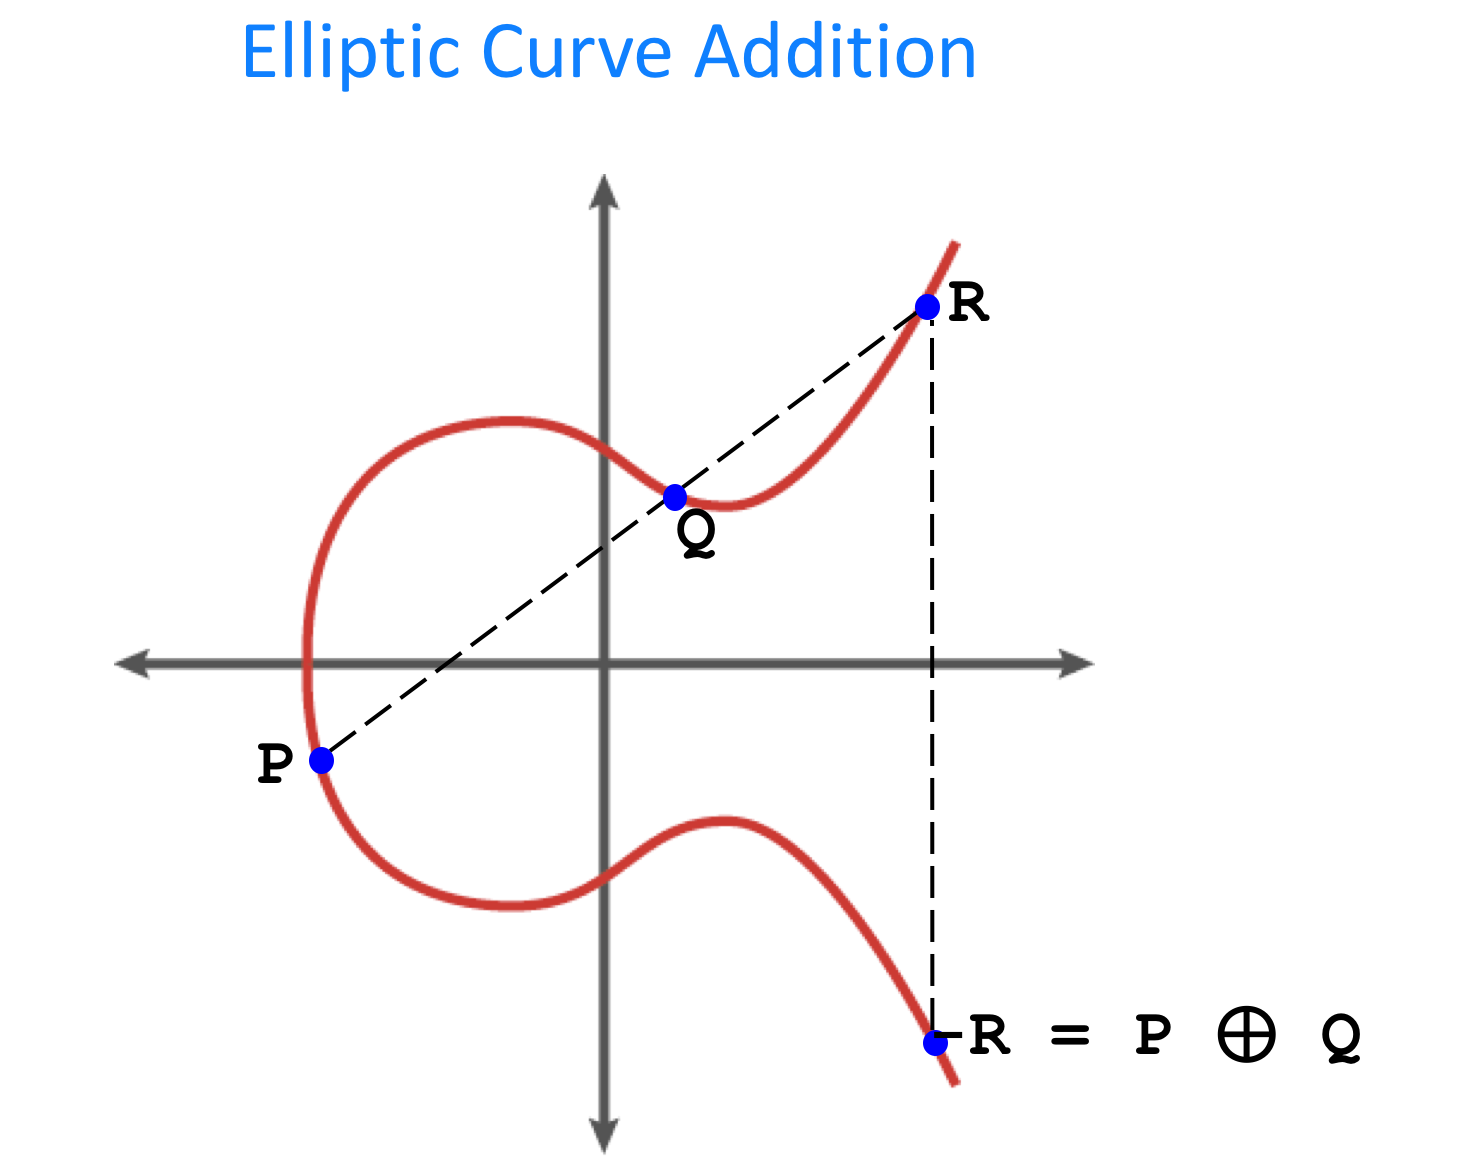
\includegraphics[width=0.75\textwidth]{images/weierstrass}.
\end{frame}


\begin{frame}{Easy to prove?}
\begin{itemize}
\item Silvermann and Tate: Rational points on elliptic curves, 1992
\vspace{0.5cm}

\begin{quote}
Of course, there are an awful lot of special cases to consider, such as when one of the points is the negative of
the other or two of the points coincide. But in a few days,
you will be able to check associativity using these formulas. So we need say nothing more about the proof of the
associative law!
\end{quote}

\item Russinoff: A Computationally Surveyable Proof of the Group Properties of an Elliptic Curve (2017).
\vspace{0.5cm}

\begin{quote}
Expanding the resulting polynomial equation into monomials would involve some $10^{25}$ terms...
\end{quote}

\end{itemize}
\end{frame}

\begin{frame}
Th\'ery, Proving the group law of elliptic curves formally (2007): 
\vspace{1cm}

\begin{quote}
To translate this 7 page long paper proof in a theorem
prover was a real challenge. In fact, the proof relies on
some non-trivial computations that the author advises to
check using a computer algebra system such as CoCoA.
The main difficulty has been to find an effective way to
cope with these computations inside our proof system.
\end{quote}
\end{frame}

\section{Affine Edwards curves}

\begin{frame}{Affine Edwards curves}
\begin{itemize}
	\setlength\itemsep{2em}
	\item Let $k$ be an arbitrary field and $c,d,x,y \in k$ with $c,d$ fixed.
	\item An affine Edwards curve is given by the set of zeros of the polynomial: \[e(x,y) = x^2 + cy^2 - 1 - d x^2y^2\]
	\item The following addition determines a group law on the curve: \[(x_1,y_1) \oplus_0 (x_2,y_2) = \Big(\frac{x_1x_2-cy_1y_2}{1-dx_1x_2y_1y_1},\frac{x_1y_2+y_1 y_2}{1+d x_1 x_2 y_1y_2}\Big)\]
\end{itemize}
% Añadir pausas
\end{frame}

\begin{frame}{Geometric interpretation}
\begin{figure}
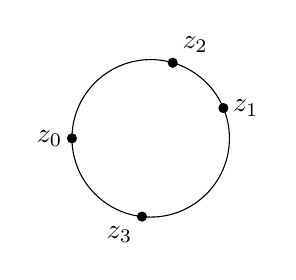
\begin{tikzpicture}
\draw (0,0) circle (1);
\draw plot[smooth] file {figC1.table};
\draw plot[smooth] file {figC2.table};
\smalldot {-1,0} node[anchor=east] {$z_0$};
\smalldot {12/13,5/13} node[anchor=west] {$z_1$};
\smalldot {7/25,24/25} node[anchor=south west] {$z_2$};
\smalldot {-36/325,-323/325} node[anchor=north east] {$z_3$};
\end{tikzpicture}
\end{figure}
\begin{figure}
\begin{tikzpicture}
\draw plot[smooth] file {figE1.table};
\draw plot[smooth] file {figE2.table};
\draw plot[smooth] file {figE3.table};
\draw plot[smooth] file {figE4.table};
\smalldot {-1,0} node[anchor=east] {$z_0$};
\smalldot {0.9,0.158} node[anchor=west] {$z_1$};
\smalldot {0.2,0.853} node[anchor=south west] {$z_2$};
\smalldot {0.037,-0.993} node[anchor=north east] {$z_3$};
\end{tikzpicture}	
\end{figure}
\hspace*{10pt}\hbox{\scriptsize Source: Thomas Hales, The Group Law for Edwards Curves (2016)}
\end{frame}

\begin{frame}{Affine statement}
% put in a proper environment
\begin{theorem}[group law]
	If $c$ is a square and $
	d \neq 0$ is not a square, then:  
	\[
	C= \{(x,y)\in k^2 \mid  e(x,y) = 0\}
	\]
	is an abelian group with binary operation $\oplus_0$.
\end{theorem}
\end{frame}

\begin{frame}{The group law in Isabelle/HOL}
% Put pauses
\begin{itemize}
\item Associativity is the hardest to prove. 
%\begin{figure} {%
	
\begin{isabellebody}%

add\ {\isacharcolon}{\isacharcolon}\ {\isacharprime}a\ {\isasymtimes}\ {\isacharprime}a\ {\isasymRightarrow}\ {\isacharprime}a\ {\isasymtimes}\ {\isacharprime}a\ {\isasymRightarrow}\ {\isacharprime}a\ {\isasymtimes}\ {\isacharprime}a\ \isanewline
add\ {\isacharparenleft}x\isactrlsub {\isadigit{1}}{\isacharcomma}y\isactrlsub {\isadigit{1}}{\isacharparenright}\ {\isacharparenleft}x\isactrlsub {\isadigit{2}}{\isacharcomma}y\isactrlsub {\isadigit{2}}{\isacharparenright}\ {\isacharequal}
{\isacharparenleft}{\isacharparenleft}x\isactrlsub {\isadigit{1}}{\isacharasterisk}x\isactrlsub {\isadigit{2}}\ {\isacharminus}\ c{\isacharasterisk}y\isactrlsub {\isadigit{1}}{\isacharasterisk}y\isactrlsub {\isadigit{2}}{\isacharparenright}\ div {\isacharparenleft}{\isadigit{1}}{\isacharminus}d{\isacharasterisk}x\isactrlsub {\isadigit{1}}{\isacharasterisk}y\isactrlsub {\isadigit{1}}{\isacharasterisk}x\isactrlsub {\isadigit{2}}{\isacharasterisk}y\isactrlsub {\isadigit{2}}{\isacharparenright}{\isacharcomma}\ \isanewline
\ \ \ \ \ \ \ \ \ \ \ \ \ \ \ \ \ \ \ \ \ \ \ {\isacharparenleft}x\isactrlsub {\isadigit{1}}{\isacharasterisk}y\isactrlsub {\isadigit{2}}{\isacharplus}y\isactrlsub {\isadigit{1}}{\isacharasterisk}x\isactrlsub {\isadigit{2}}{\isacharparenright}\ div\ {\isacharparenleft}{\isadigit{1}}{\isacharplus}d{\isacharasterisk}x\isactrlsub {\isadigit{1}}{\isacharasterisk}y\isactrlsub {\isadigit{1}}{\isacharasterisk}x\isactrlsub {\isadigit{2}}{\isacharasterisk}y\isactrlsub {\isadigit{2}}{\isacharparenright}{\isacharparenright}
\end{isabellebody}%



%:%file=~/Isabelle/curves_safe/Hales.thy%:%
%:%10=1%:%
%:%11=1%:%
%:%12=2%:%
%:%13=3%:%
%:%18=3%:%
%:%21=4%:%
%:%22=5%:%
%:%23=5%:%
%:%30=8%:%
%:%40=10%:%
%:%41=10%:%
%:%42=11%:%
%:%43=12%:%
%:%44=13%:%
%:%45=13%:%
%:%46=14%:%
%:%47=15%:%
%:%48=16%:%
%:%49=17%:%
%:%50=17%:%
%:%51=18%:%
%:%53=20%:%
%:%54=21%:%
%:%55=22%:%
%:%56=22%:%
%:%57=23%:%
%:%58=24%:%
%:%59=25%:%
%:%60=25%:%
%:%61=26%:%
%:%62=27%:%
%:%63=28%:%
%:%64=28%:%
%:%65=29%:%
%:%66=30%:%
%:%67=31%:%
%:%68=32%:%
%:%69=32%:%
%:%70=33%:%
%:%71=34%:%
%:%72=35%:%
%:%73=35%:%
%:%74=36%:%
%:%75=37%:%
%:%76=38%:%
%:%77=39%:%
%:%78=40%:%
%:%79=41%:%
%:%80=42%:%
%:%81=43%:%
%:%88=44%:%
%:%89=44%:%
%:%90=45%:%
%:%91=45%:%
%:%92=46%:%
%:%93=46%:%
%:%94=47%:%
%:%95=47%:%
%:%96=48%:%
%:%97=48%:%
%:%99=50%:%
%:%100=51%:%
%:%101=51%:%
%:%103=53%:%
%:%104=54%:%
%:%105=54%:%
%:%106=55%:%
%:%107=55%:%
%:%108=56%:%
%:%109=56%:%
%:%110=57%:%
%:%111=57%:%
%:%112=58%:%
%:%113=59%:%
%:%114=59%:%
%:%115=60%:%
%:%116=60%:%
%:%117=60%:%
%:%118=61%:%
%:%119=61%:%
%:%120=62%:%
%:%121=62%:%
%:%122=62%:%
%:%123=63%:%
%:%124=63%:%
%:%125=64%:%
%:%126=64%:%
%:%127=64%:%
%:%128=65%:%
%:%129=65%:%
%:%130=66%:%
%:%131=66%:%
%:%132=66%:%
%:%133=67%:%
%:%134=68%:%
%:%135=68%:%
%:%136=69%:%
%:%137=69%:%
%:%138=69%:%
%:%139=70%:%
%:%140=71%:%
%:%141=71%:%
%:%148=78%:%
%:%149=79%:%
%:%150=79%:%
%:%151=80%:%
%:%152=80%:%
%:%153=81%:%
%:%154=81%:%
%:%155=82%:%
%:%156=82%:%
%:%157=83%:%
%:%158=83%:%
%:%159=84%:%
%:%160=85%:%
%:%161=85%:%
%:%162=86%:%
%:%167=91%:%
%:%168=92%:%
%:%169=92%:%
%:%170=93%:%
%:%171=93%:%
%:%172=94%:%
%:%173=94%:%
%:%174=95%:%
%:%175=95%:%
%:%176=96%:%
%:%177=96%:%
%:%178=97%:%
%:%179=98%:%
%:%180=98%:%
%:%181=99%:%
%:%182=99%:%
%:%183=100%:%
%:%184=100%:%
%:%185=101%:%
%:%186=101%:%
%:%187=102%:%
%:%188=102%:%
%:%189=103%:%
%:%190=103%:%
%:%191=104%:%
%:%192=104%:%
%:%193=105%:%
%:%194=105%:%
%:%195=106%:%
%:%196=107%:%
%:%197=107%:%
%:%198=108%:%
%:%199=109%:%
%:%200=109%:%
%:%201=109%:%
%:%202=110%:%
%:%203=110%:%
%:%204=111%:%
%:%205=112%:%
%:%211=112%:%
%:%214=113%:%
%:%215=114%:%
%:%223=118%:%
%:%233=120%:%
%:%234=120%:%
%:%235=121%:%
%:%236=122%:%
%:%237=123%:%
%:%238=124%:%
%:%239=125%:%
%:%240=126%:%
%:%241=127%:%
%:%242=127%:%
%:%243=128%:%
%:%245=130%:%
%:%246=131%:%
%:%247=132%:%
%:%248=132%:%
%:%249=133%:%
%:%250=134%:%
%:%251=134%:%
%:%252=135%:%
%:%253=136%:%
%:%254=137%:%
%:%255=138%:%
%:%256=139%:%
%:%257=140%:%
%:%258=140%:%
%:%259=141%:%
%:%260=142%:%
%:%261=142%:%
%:%262=143%:%
%:%263=144%:%
%:%264=144%:%
%:%265=145%:%
%:%266=146%:%
%:%267=147%:%
%:%268=147%:%
%:%269=148%:%
%:%270=149%:%
%:%271=149%:%
%:%272=150%:%
%:%273=151%:%
%:%274=151%:%
%:%275=152%:%
%:%278=155%:%
%:%279=156%:%
%:%280=157%:%
%:%281=158%:%
%:%282=158%:%
%:%283=159%:%
%:%284=160%:%
%:%285=161%:%
%:%288=162%:%
%:%292=162%:%
%:%298=162%:%
%:%301=163%:%
%:%302=164%:%
%:%303=164%:%
%:%304=165%:%
%:%305=166%:%
%:%306=166%:%
%:%307=167%:%
%:%308=168%:%
%:%309=169%:%
%:%310=170%:%
%:%313=171%:%
%:%317=171%:%
%:%323=171%:%
%:%326=172%:%
%:%327=173%:%
%:%328=173%:%
%:%330=173%:%
%:%334=173%:%
%:%335=173%:%
%:%336=173%:%
%:%343=173%:%
%:%344=174%:%
%:%345=175%:%
%:%346=175%:%
%:%347=176%:%
%:%349=178%:%
%:%350=179%:%
%:%351=180%:%
%:%352=180%:%
%:%353=181%:%
%:%355=183%:%
%:%356=184%:%
%:%357=185%:%
%:%358=185%:%
%:%359=186%:%
%:%360=187%:%
%:%361=188%:%
%:%362=189%:%
%:%363=189%:%
%:%364=190%:%
%:%365=191%:%
%:%366=192%:%
%:%367=192%:%
%:%368=193%:%
%:%369=194%:%
%:%370=195%:%
%:%379=204%:%
%:%380=205%:%
%:%383=206%:%
%:%387=206%:%
%:%393=206%:%
%:%396=207%:%
%:%397=208%:%
%:%398=208%:%
%:%400=208%:%
%:%404=208%:%
%:%405=208%:%
%:%406=208%:%
%:%413=208%:%
%:%414=209%:%
%:%415=210%:%
%:%416=210%:%
%:%417=211%:%
%:%418=212%:%
%:%419=213%:%
%:%420=214%:%
%:%421=215%:%
%:%422=216%:%
%:%423=217%:%
%:%424=217%:%
%:%427=218%:%
%:%432=219%:%} \end{figure}
\item $
e_i = x_i^2 + c *
y_i^2 - 1 - d * x_i^2 * y_i^2 = 0
$
\item Normalized associativity equation: $
\text{gxpoly} = ((p_1 \oplus_0 p_2)
\oplus_0 p_3 - p_1 \oplus_0 (p_2 \oplus_0 p_3))_1*\Delta_x
$

%\item Since points are \emph{summable}, $\Delta_x \neq 0$. 
\end{itemize}
\vspace{0.5cm}
%
	
\begin{isabellebody}%

\ \ \isacommand{have}\isamarkupfalse%
\ {\isachardoublequoteopen}{\isasymexists}\ r{\isadigit{1}}\ r{\isadigit{2}}\ r{\isadigit{3}}{\isachardot}\ gxpoly\ {\isacharequal}\ r{\isadigit{1}}\ {\isacharasterisk}\ e{\isadigit{1}}\ {\isacharplus}\ r{\isadigit{2}}\ {\isacharasterisk}\ e{\isadigit{2}}\ {\isacharplus}\ r{\isadigit{3}}\ {\isacharasterisk}\ e{\isadigit{3}}{\isachardoublequoteclose}\isanewline
\ \ \ \ \isacommand{unfolding}\isamarkupfalse%
\ gxpoly{\isacharunderscore}def\ Delta\isactrlsub x{\isacharunderscore}def\ \isanewline
\ \ \ \ \isacommand{apply}\isamarkupfalse%
{\isacharparenleft}simp\ add{\isacharcolon}\ assms{\isacharparenleft}{\isadigit{1}}{\isacharcomma}{\isadigit{2}}{\isacharparenright}{\isacharparenright}\isanewline
\ \ \ \ \isacommand{apply}\isamarkupfalse%
{\isacharparenleft}rewrite\ \isakeyword{in}\ {\isachardoublequoteopen}{\isacharunderscore}\ {\isacharslash}\ {\isasymhole}{\isachardoublequoteclose}\ delta{\isacharunderscore}minus{\isacharunderscore}def{\isacharbrackleft}symmetric{\isacharbrackright}{\isacharparenright}{\isacharplus}\isanewline
\ \ \ \ \isacommand{apply}\isamarkupfalse%
{\isacharparenleft}simp\ add{\isacharcolon}\ divide{\isacharunderscore}simps\ assms{\isacharparenleft}{\isadigit{9}}{\isacharcomma}{\isadigit{1}}{\isadigit{1}}{\isacharparenright}{\isacharparenright}\isanewline
\ \ \ \ \isacommand{apply}\isamarkupfalse%
{\isacharparenleft}rewrite\ left{\isacharunderscore}diff{\isacharunderscore}distrib{\isacharparenright}\isanewline
\ \ \ \ \isacommand{apply}\isamarkupfalse%
{\isacharparenleft}simp\ add{\isacharcolon}\ simp{\isadigit{1}}gx\ simp{\isadigit{2}}gx{\isacharparenright}\isanewline
\ \ \ \ \isacommand{unfolding}\isamarkupfalse%
\ delta{\isacharunderscore}plus{\isacharunderscore}def\ delta{\isacharunderscore}minus{\isacharunderscore}def\isanewline
\ \ \ \ \ \ \ \ \ \ \ \ \ \ e{\isadigit{1}}{\isacharunderscore}def\ e{\isadigit{2}}{\isacharunderscore}def\ e{\isadigit{3}}{\isacharunderscore}def\ e{\isacharunderscore}def\isanewline
\ \ \ \ \isacommand{by}\isamarkupfalse%
\ algebra\isanewline

\end{isabellebody}%



%:%file=~/Isabelle/curves_safe/Hales.thy%:%
%:%10=1%:%
%:%11=1%:%
%:%12=2%:%
%:%13=3%:%
%:%18=3%:%
%:%21=4%:%
%:%22=5%:%
%:%23=5%:%
%:%30=8%:%
%:%40=10%:%
%:%41=10%:%
%:%42=11%:%
%:%43=12%:%
%:%44=13%:%
%:%45=13%:%
%:%46=14%:%
%:%47=15%:%
%:%48=16%:%
%:%49=17%:%
%:%50=17%:%
%:%51=18%:%
%:%53=20%:%
%:%54=21%:%
%:%55=22%:%
%:%56=22%:%
%:%57=23%:%
%:%58=24%:%
%:%59=25%:%
%:%60=25%:%
%:%61=26%:%
%:%62=27%:%
%:%63=28%:%
%:%64=28%:%
%:%65=29%:%
%:%66=30%:%
%:%67=31%:%
%:%68=32%:%
%:%69=32%:%
%:%70=33%:%
%:%71=34%:%
%:%72=35%:%
%:%73=35%:%
%:%74=36%:%
%:%75=37%:%
%:%76=38%:%
%:%77=39%:%
%:%78=40%:%
%:%79=41%:%
%:%80=42%:%
%:%81=43%:%
%:%88=44%:%
%:%89=44%:%
%:%90=45%:%
%:%91=45%:%
%:%92=46%:%
%:%93=46%:%
%:%94=47%:%
%:%95=47%:%
%:%96=48%:%
%:%97=48%:%
%:%99=50%:%
%:%100=51%:%
%:%101=51%:%
%:%103=53%:%
%:%104=54%:%
%:%105=54%:%
%:%106=55%:%
%:%107=55%:%
%:%108=56%:%
%:%109=56%:%
%:%110=57%:%
%:%111=57%:%
%:%112=58%:%
%:%113=59%:%
%:%114=59%:%
%:%115=60%:%
%:%116=60%:%
%:%117=60%:%
%:%118=61%:%
%:%119=61%:%
%:%120=62%:%
%:%121=62%:%
%:%122=62%:%
%:%123=63%:%
%:%124=63%:%
%:%125=64%:%
%:%126=64%:%
%:%127=64%:%
%:%128=65%:%
%:%129=65%:%
%:%130=66%:%
%:%131=66%:%
%:%132=66%:%
%:%133=67%:%
%:%134=68%:%
%:%135=68%:%
%:%136=69%:%
%:%137=69%:%
%:%138=69%:%
%:%139=70%:%
%:%140=71%:%
%:%141=71%:%
%:%148=78%:%
%:%149=79%:%
%:%150=79%:%
%:%151=80%:%
%:%152=80%:%
%:%153=81%:%
%:%154=81%:%
%:%155=82%:%
%:%156=82%:%
%:%157=83%:%
%:%158=83%:%
%:%159=84%:%
%:%160=85%:%
%:%161=85%:%
%:%162=86%:%
%:%167=91%:%
%:%168=92%:%
%:%169=92%:%
%:%170=93%:%
%:%171=93%:%
%:%172=94%:%
%:%173=94%:%
%:%174=95%:%
%:%175=95%:%
%:%176=96%:%
%:%177=96%:%
%:%178=97%:%
%:%179=98%:%
%:%180=98%:%
%:%181=99%:%
%:%182=99%:%
%:%183=100%:%
%:%184=100%:%
%:%185=101%:%
%:%186=101%:%
%:%187=102%:%
%:%188=102%:%
%:%189=103%:%
%:%190=103%:%
%:%191=104%:%
%:%192=104%:%
%:%193=105%:%
%:%194=105%:%
%:%195=106%:%
%:%196=107%:%
%:%197=107%:%
%:%198=108%:%
%:%199=109%:%
%:%200=109%:%
%:%201=109%:%
%:%202=110%:%
%:%203=110%:%
%:%204=111%:%
%:%205=112%:%
%:%211=112%:%
%:%214=113%:%
%:%215=114%:%
%:%223=118%:%
%:%233=120%:%
%:%234=120%:%
%:%235=121%:%
%:%236=122%:%
%:%237=123%:%
%:%238=124%:%
%:%239=125%:%
%:%240=126%:%
%:%241=127%:%
%:%242=127%:%
%:%243=128%:%
%:%245=130%:%
%:%246=131%:%
%:%247=132%:%
%:%248=132%:%
%:%249=133%:%
%:%250=134%:%
%:%251=134%:%
%:%252=135%:%
%:%253=136%:%
%:%254=137%:%
%:%255=138%:%
%:%256=139%:%
%:%257=140%:%
%:%258=140%:%
%:%259=141%:%
%:%260=142%:%
%:%261=142%:%
%:%262=143%:%
%:%263=144%:%
%:%264=144%:%
%:%265=145%:%
%:%266=146%:%
%:%267=147%:%
%:%268=147%:%
%:%269=148%:%
%:%270=149%:%
%:%271=149%:%
%:%272=150%:%
%:%273=151%:%
%:%274=151%:%
%:%275=152%:%
%:%278=155%:%
%:%279=156%:%
%:%280=157%:%
%:%281=158%:%
%:%282=158%:%
%:%283=159%:%
%:%284=160%:%
%:%285=161%:%
%:%288=162%:%
%:%292=162%:%
%:%298=162%:%
%:%301=163%:%
%:%302=164%:%
%:%303=164%:%
%:%304=165%:%
%:%305=166%:%
%:%306=166%:%
%:%307=167%:%
%:%308=168%:%
%:%309=169%:%
%:%310=170%:%
%:%313=171%:%
%:%317=171%:%
%:%323=171%:%
%:%326=172%:%
%:%327=173%:%
%:%328=173%:%
%:%330=173%:%
%:%334=173%:%
%:%335=173%:%
%:%336=173%:%
%:%343=173%:%
%:%344=174%:%
%:%345=175%:%
%:%346=175%:%
%:%347=176%:%
%:%349=178%:%
%:%350=179%:%
%:%351=180%:%
%:%352=180%:%
%:%353=181%:%
%:%355=183%:%
%:%356=184%:%
%:%357=185%:%
%:%358=185%:%
%:%359=186%:%
%:%360=187%:%
%:%361=188%:%
%:%362=189%:%
%:%363=189%:%
%:%364=190%:%
%:%365=191%:%
%:%366=192%:%
%:%367=192%:%
%:%368=193%:%
%:%369=194%:%
%:%370=195%:%
%:%379=204%:%
%:%380=205%:%
%:%383=206%:%
%:%387=206%:%
%:%393=206%:%
%:%396=207%:%
%:%397=208%:%
%:%398=208%:%
%:%400=208%:%
%:%404=208%:%
%:%405=208%:%
%:%406=208%:%
%:%413=208%:%
%:%414=209%:%
%:%415=210%:%
%:%416=210%:%
%:%417=211%:%
%:%418=212%:%
%:%419=213%:%
%:%420=214%:%
%:%421=215%:%
%:%422=216%:%
%:%423=217%:%
%:%424=217%:%
%:%427=218%:%
%:%432=219%:%

\begin{itemize}
	\item Like Mathematica but without explicitly computing $r_i$.
\end{itemize}
% Do a live demostration
\end{frame}

\begin{frame}{Key tools}
\begin{itemize}
	\item The \emph{rewrite} tactic: rewrites in subterms specified by a pattern.
	
	\item The \textit{algebra} method: given
	$e_i(x),\ p_{ij}(x),\ a_i(x) \in R[x_1,\ldots,x_n]$, where $R$ is a
	commutative ring and $x=(x_1,\ldots,x_n)$, the method checks formulas:
	\[
	\; \forall x.\ \bigwedge_{i = 1}^L
	e_i({x}) = 0 \to \exists{y}.\ \bigwedge_{i = 1}^M
	\left(a_i(x) = \sum_{j = 1}^N p_{ij}({x}) y_j \right)
	\] 
	The method is complete for formulas holding over all commutative rings with unit.
	
	\item In particular, ideal membership problems fit in this formula.
\end{itemize}
\end{frame}

\section{Projective Edwards Curves}

\begin{frame}{Projective Edwards curves}
\begin{itemize}
	\item Bypass restriction: $d$ not a non-null square. 
	\item Assume $c \neq 0$ and $c,d$ are squares.
	\item Set $t^2 = \frac d c$ and change variables $y \mapsto \frac y c$ to get: \[e(x,y) = x^2+y^2-1-t^2x^2y^2\]
	\item Define a second addition $\oplus_1$: \[(x_1,y_1) \oplus_1 (x_2,y_2) = \Big(\frac{x_1y_1-x_2y_2}{x_2y_1 - x_1y_2},\frac{x_1y_1+x_2 y_2}{x_1 x_2 + y_1y_2}\Big)\]
\end{itemize}	
\vspace{0.5cm}
\pause
\begin{itemize}	
	\item Define $E_{\text{aff}}$ (points on curve) and $E^{\circ}$ (non-zero coordinates)
	\item Make two copies of $E_{aff}$. $(P,i)$ is representative of $P$ on i-th copy.
	\item For $P \in E^{\circ}$, identify $(P,i) \sim (\tau P, i+1)$.
	\item Let $E = E_{aff}^2 / \sim$ be the quotient set with elements $[P,i]$.
	\item Define addition on $E$ as: \[[P,i] \oplus [Q,j] = [P \oplus_l Q, i+j]\] if $\delta_l(P,Q) \neq 0, l \in \mathbb{F}_2 = \{0,1\}$. 
\end{itemize}
\end{frame}


\begin{frame}{Projective addition in Isabelle/HOL}
\begin{itemize}
	\item Definition as usual:
	\vspace{0.25cm}
	\begin{enumerate}
		\setlength\itemsep{0.75em}
		\item Basic operation: add $((x_1,y_1),i)$ and $((x_2,y_2),j)$.
		\item Apply basic operation to all pairs from two classes $c_1,c_2$.
		\item Apply the equivalence relation $\sim$.
		\item Extract the resulting class $c_1 \oplus c_2$.
	\end{enumerate}
\end{itemize}
\vspace{0.5cm}
\pause
\begin{itemize}	
	\item This uses Isabelle's ability to encode \textbf{partial functions}.
	\item The resulting definition is \textbf{easy to compute}. The equivalence classes are:
	\[[(x,y),i] = 
	\begin{cases}
	\{ ((x,y),i) \} & x = 0 \lor y = 0 \\
	\{ ((x,y),i), (\tau (x,y),i+1) \} & x \neq 0 \land y \neq 0
	\end{cases}\]
	for $(x,y) \in E_{aff}$.
	\item But! Prove the \textbf{independence of the representative}. 
\end{itemize}
\end{frame}

\begin{frame}{Using Isabelle's Gr\"obner basis}
\begin{itemize}
	\item \textbf{Dichotomy:} if $P,Q \in E_{aff}$ then 
	
	\begin{itemize}
		\item $P \in E^{\circ}$ and $Q = g i P$ for some $g \in \tau \langle \rho \rangle$, or
		\item $(P, Q) \in E_{aff,i}$ for some $i$.
	\end{itemize}
	
	\item \textbf{Proof:} solve particular ideal membership problems.
	\item Formalization caught some \textbf{misinterpretation of computer algebra calculations}:	
	\[
	\exists r_1 \, r_2 \, r_3 \, r_4.\ 
	y_0^2 - x_1^2 = r_1 e(x_0,y_0) + r_2 e(x_1,y_1) + r_3 \delta' + r_4
	\delta_{-} 
	\] 
	corrected to:
	\[
	\exists r_1 \, r_2 \, r_3 \, r_4.\ 
	2 x_0 y_0 (y_0^2 - x_1^2) = r_1 e(x_0,y_0) + r_2 e(x_1,y_1) + r_3 \delta' + r_4
	\delta_{-}
	\]
	\item In other case, some \textbf{strengthening of the hypothesis} needed:
	
	$\delta_{+} = 0$ to $\delta_{-} \neq 0$
	
	\item We also produced a proof without Gr\"obner basis. 
\end{itemize}
\end{frame}

\begin{frame}{When the assistant shows you the proof ($\delta$-relations)}

First findings, used for the independence of class representative:

\begin{table}
	\begin{center}
		\begin{tabular}{ r c l }
			$\delta \; \tau P_1 \; \tau P_2 \neq 0$
			& $\implies$ & $\; \delta \; P_1 \; P_2 \neq 0$ \\ 
			$\delta' \; \tau P_1 \; \tau P_2 \neq 0$
			& $\implies$ & $\; \delta' \; P_1 \; P_2 \neq 0$ \\ 
			$\delta \; P_1 \; P_2 \neq 0$,\quad $\; \delta \; P_1 \; \tau P_2 \neq 0$
			& $\implies$ & $\delta' \; P_1 \; P_2 \neq 0$ \\ 
			$\delta' \; P_1 \; P_2 \neq 0$,\quad $\; \delta' \; P_1 \; \tau P_2 \neq 0$
			& $\implies$ & $\delta \; P_1 \;P_2 \neq 0$ \\
		\end{tabular}
	\end{center}
\end{table}

Natural to ask about sums. Crucial to establish associativity:

\begin{table}
	\begin{center}
		\begin{tabular}{ r c l }
			$\delta' \; (P_1 \oplus_1 P_2) \; \tau \iota P_2 \neq 0$
			& $\implies$ & $\; \delta \; (P_1 \oplus_1 P_2) \; \iota P_2 \neq 0$ \\ 
			$\delta \; P_1 \; P_2 \neq 0$,\quad $\; \delta \; (P_1 \oplus_0 P_2) \; \tau \iota P_2 \neq 0$
			& $\implies$ & $\; \delta' (P_1 \oplus_0 P_2) \; \iota P_2 \neq 0$ \\ 
			$\delta \; P_1 \; P_2 \neq 0$,\quad $\; \delta' \; (P_0 \oplus_0 P_1) \; \tau \iota P_2 \neq 0$
			& $\implies$ & $\; \delta \; (P_0 \oplus_0 P_1) \; \iota P_2 \neq 0$ \\ 	    
			$\delta' \; P_1 \; P_2 \neq 0$,\quad $\; \delta \; (P_0 \oplus_1 P_1) \; \tau \iota P_2 \neq 0$
			& $\implies$ & $\; \delta' \; (P_0 \oplus_1 P_1) \; \iota P_2 \neq 0$ \\
		\end{tabular}
	\end{center}
\end{table}
\end{frame}

\begin{frame}{Use of $\delta$-relations}
\textbf{Goal:} show $([P, 0] \oplus [Q, 0]) \oplus [iQ, 0] = [P, 0]$
\vspace{0.5cm}
\begin{itemize}
	\setlength\itemsep{2em}
	\item After applying dichotomy three times, we arrive to: $
	([P,0] \oplus [Q,0]) \oplus [\tau \iota Q,0] =
	[(P \oplus Q) \oplus \tau \iota Q,0]
	$
	\item We are stuck since $Q$ and $\tau i Q$ are not summable. 
	\item \textbf{Sledgehammer} finds a contradiction using $\delta$-relations on $\oplus$ and hypothesis of second dichotomy.
\end{itemize}
\end{frame}

\section{Final thoughts}

\begin{frame}
\begin{itemize}
	\setlength\itemsep{2em}
	\item How to address the \textbf{maintainability} and \textbf{interoperability} of proof methods in proof-assistants (recall the \textit{algebra} method) to make the next generation \textbf{usable for mathematicians}. 
	\item Further elliptic curve formalizations: Schoof's algorithm, Hasse's theorem, elliptic curve primality testing, connection of elliptic curves and modular forms...
	% schoof's algorithm is an efficient algorithm to count points on elliptic curves over finite fields
	%  elliptic curve primality testing techniques, or elliptic curve primality proving (ECPP), are among the quickest and most widely used methods in primality proving
\end{itemize}
\end{frame}

\begin{frame}{Acknowledgements}
\begin{itemize}
	\setlength\itemsep{2em}
	\item Manuel Eberl (TUM)
	\item Prof. Thomas Hales (University of Pittsburgh)
	\item Prof. Viktor Kun\v{c}ak (EPFL)	
	\item Prof. Tobias Nipkow (TUM)
\end{itemize}
\end{frame}


\end{document}
